\begin{figure*}[!htbp]
    \centering
    % Row 1 Best One-PEACE SDR
    \begin{subfigure}[b]{0.185\textwidth}
        \centering
        \scriptsize\textbf{"The heart is beating forcefully, making a thumping sound"}
        \vspace{5.0mm}
    \end{subfigure}
    \begin{subfigure}[b]{0.185\textwidth}
        \centering
        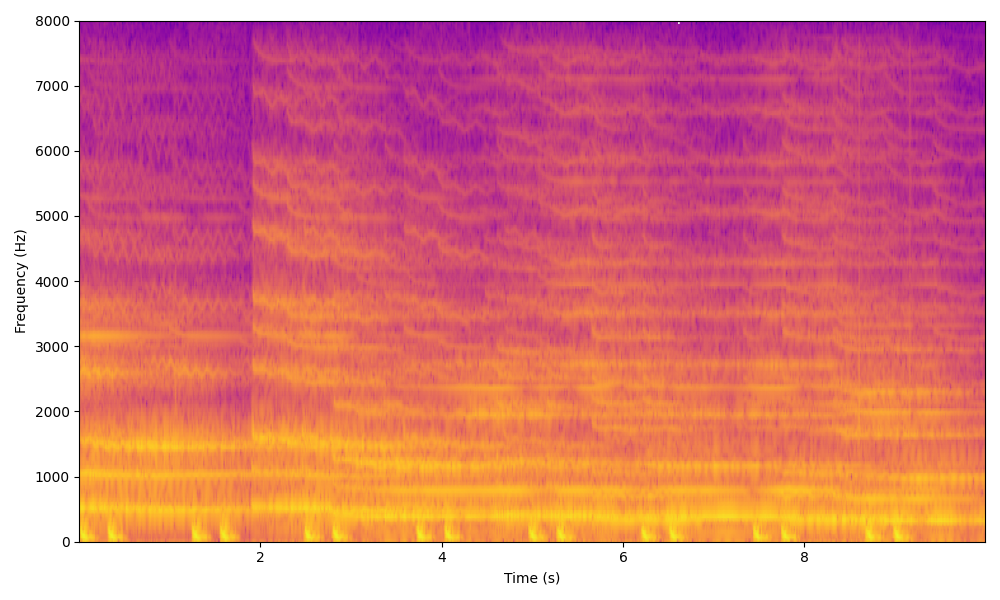
\includegraphics[width=\textwidth]{plots/onepeace_best_sdr/onepeace mixture_spectrogram.png}
    \end{subfigure}
    \begin{subfigure}[b]{0.185\textwidth}
        \centering
        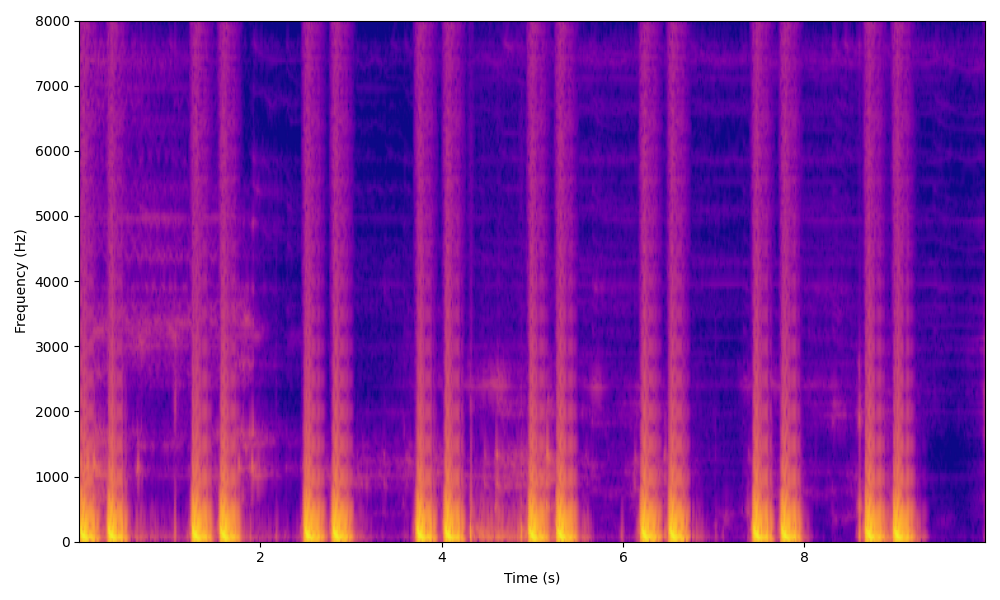
\includegraphics[width=\textwidth]{plots/onepeace_best_sdr/onepeace sep_spectrogram.png}
    \end{subfigure}
    \begin{subfigure}[b]{0.185\textwidth}
        \centering
        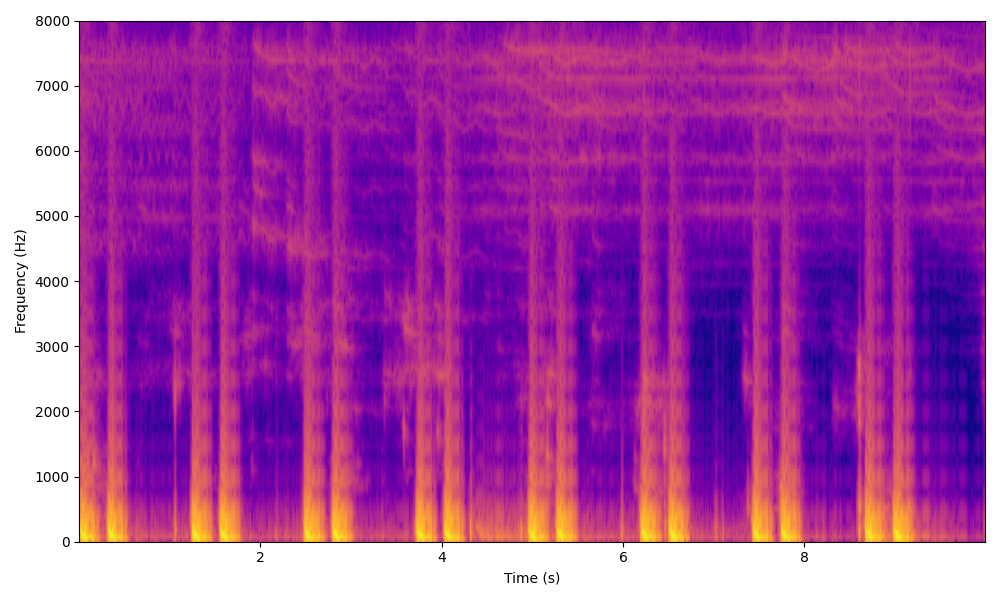
\includegraphics[width=\textwidth]{plots/onepeace_best_sdr/clap sep_spectrogram.png}
    \end{subfigure}
    \begin{subfigure}[b]{0.185\textwidth}
        \centering
        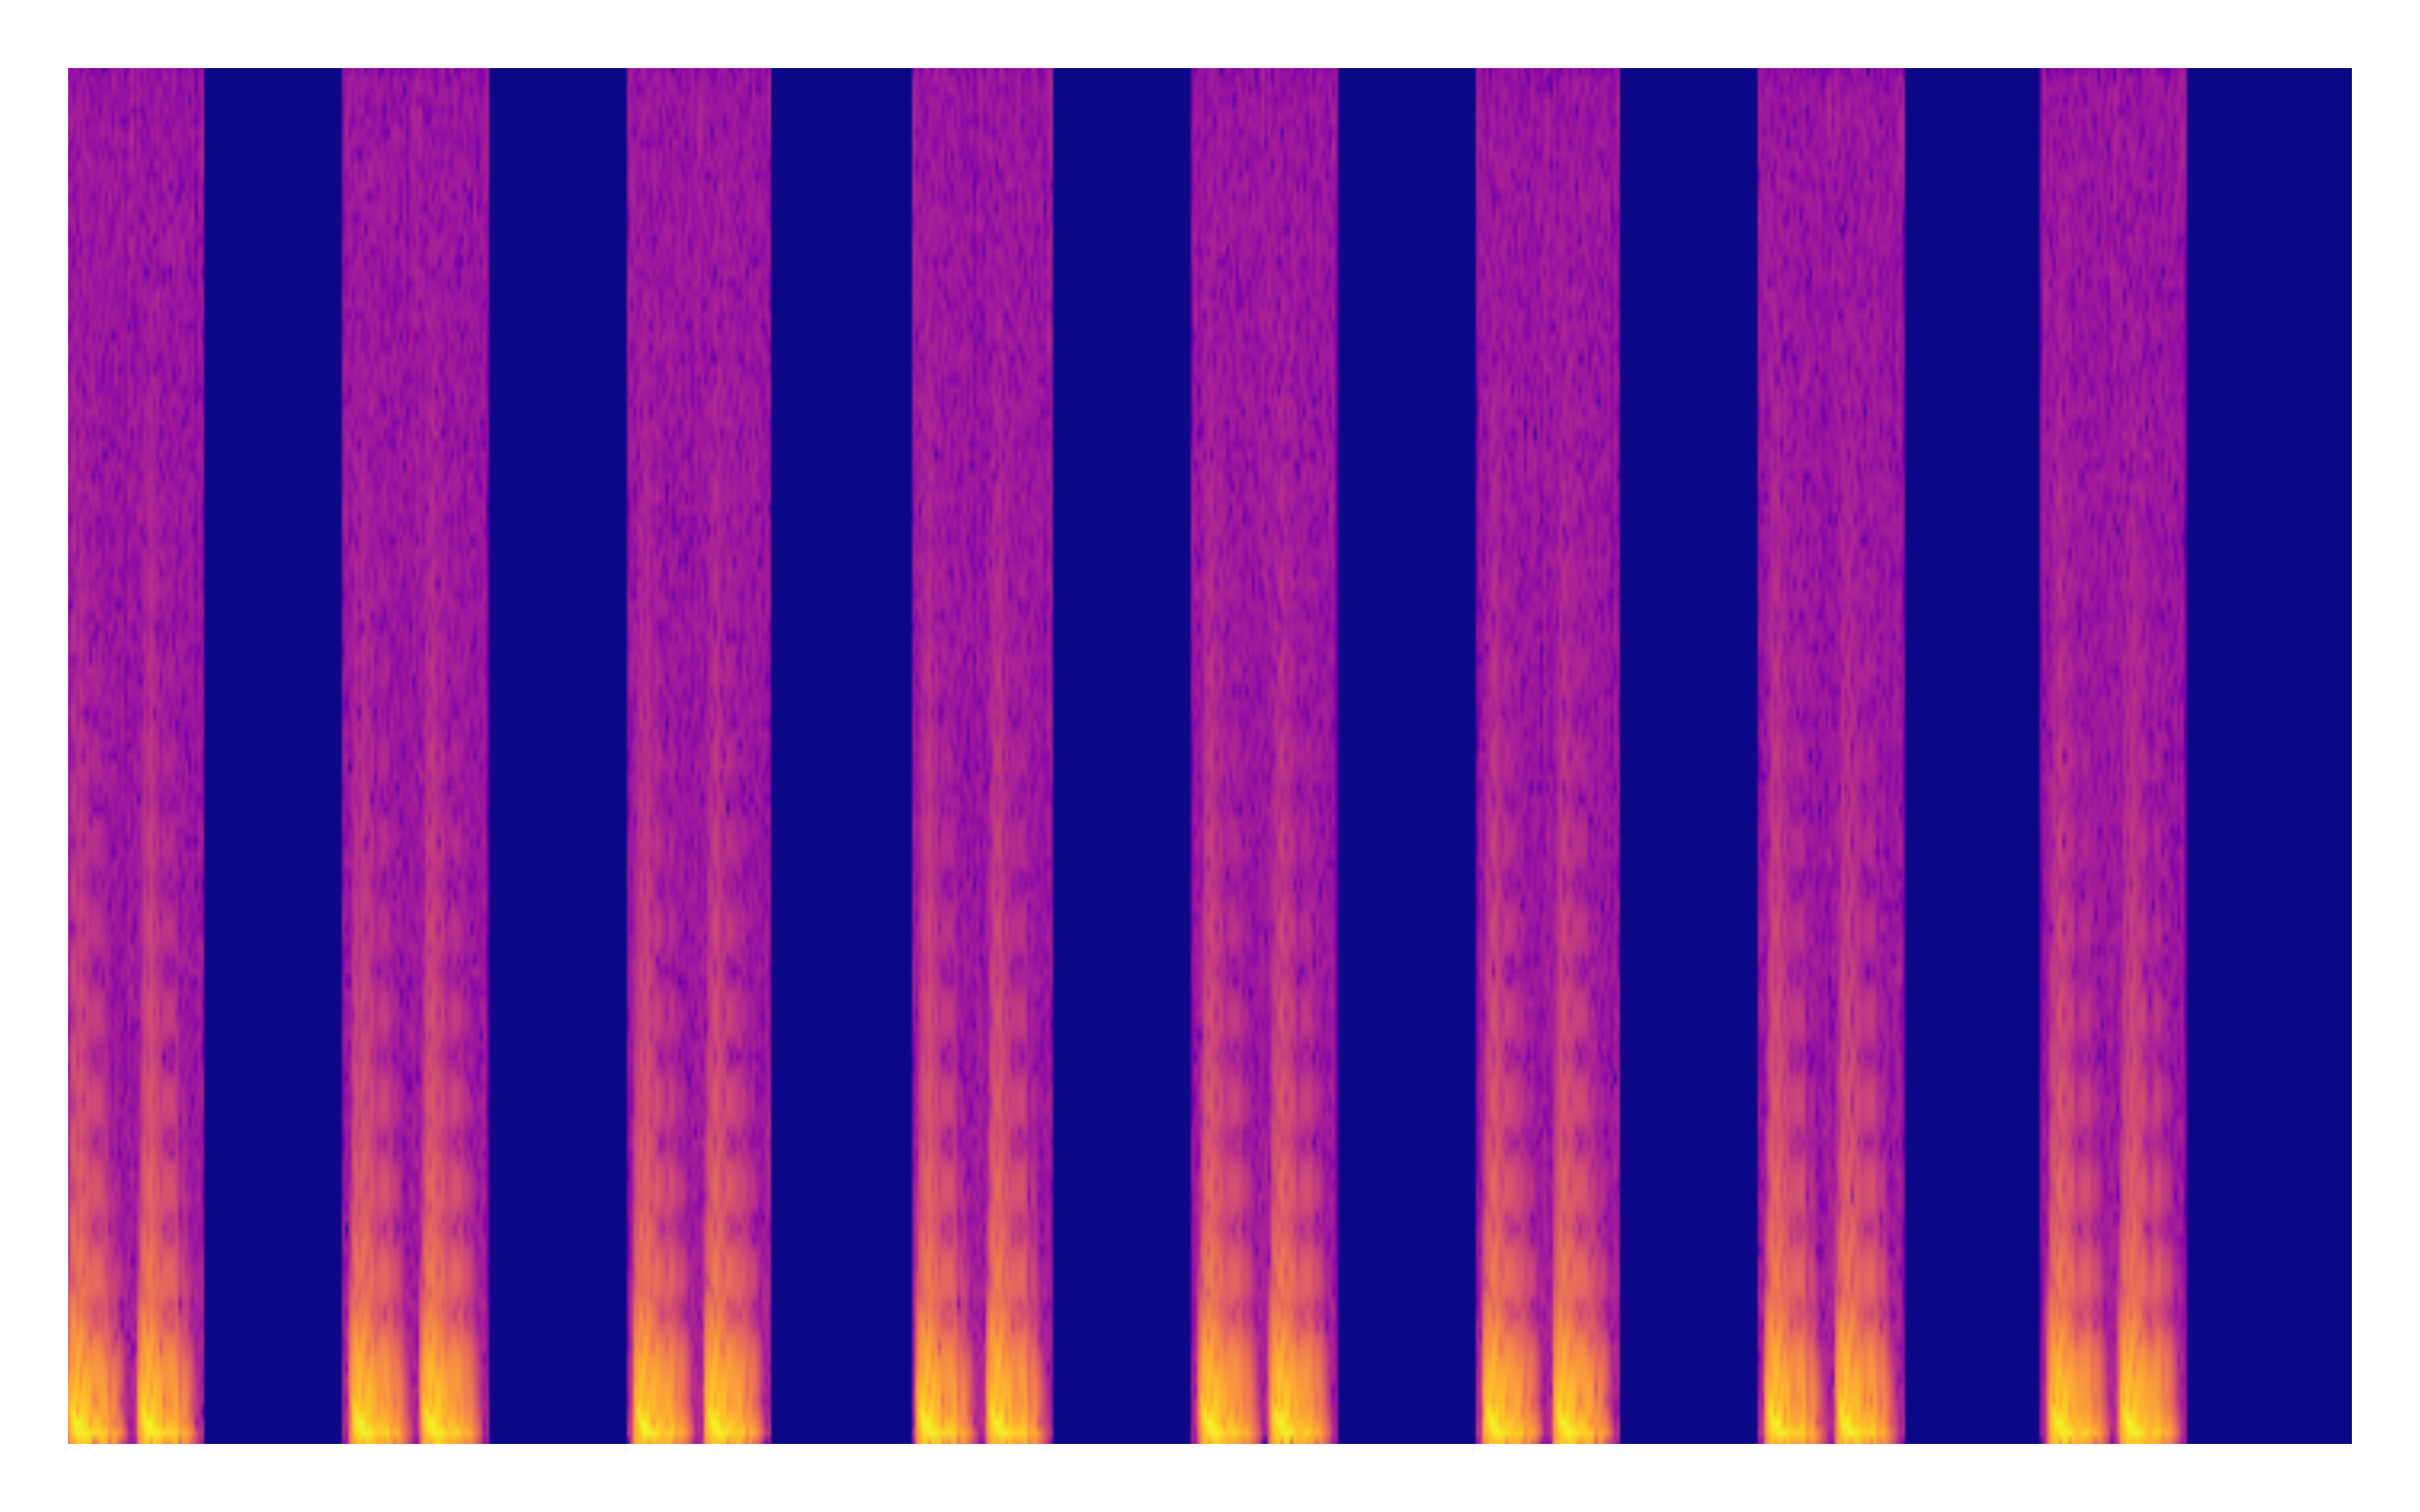
\includegraphics[width=\textwidth]{plots/onepeace_best_sdr/onepeace target_spectrogram.png}
    \end{subfigure}

    % Row 2 Best One-PEACE SDRi
    \begin{subfigure}[b]{0.185\textwidth}
        \centering
        \scriptsize\textbf{"Someone is shoveling something, making a clinking sound"}
        \vspace{5.0mm}
    \end{subfigure}
    \begin{subfigure}[b]{0.185\textwidth}
        \centering
        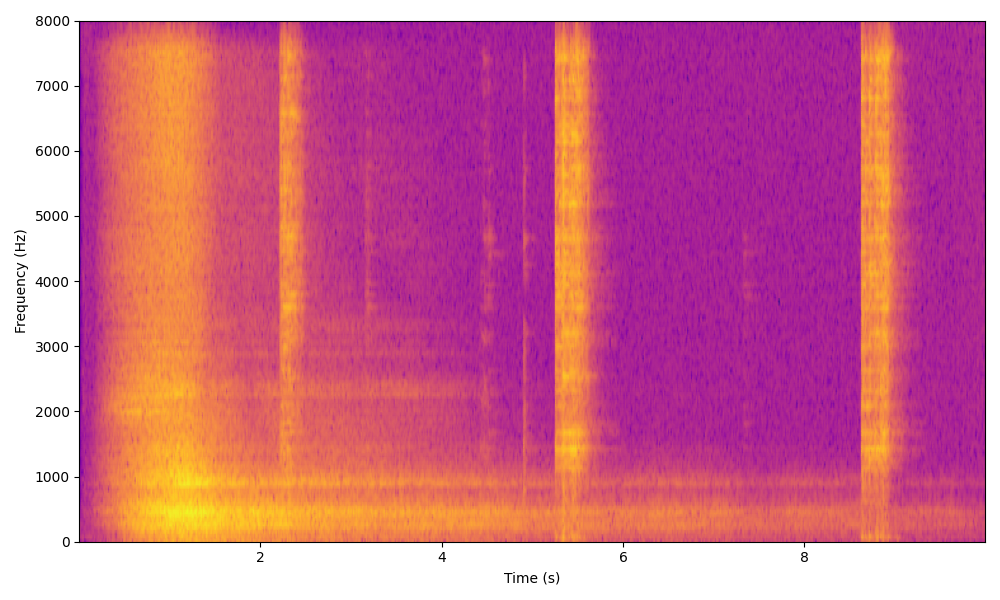
\includegraphics[width=\textwidth]{plots/onepeace_best_sdri/onepeace mixture_spectrogram.png}
    \end{subfigure}
    \begin{subfigure}[b]{0.185\textwidth}
        \centering
        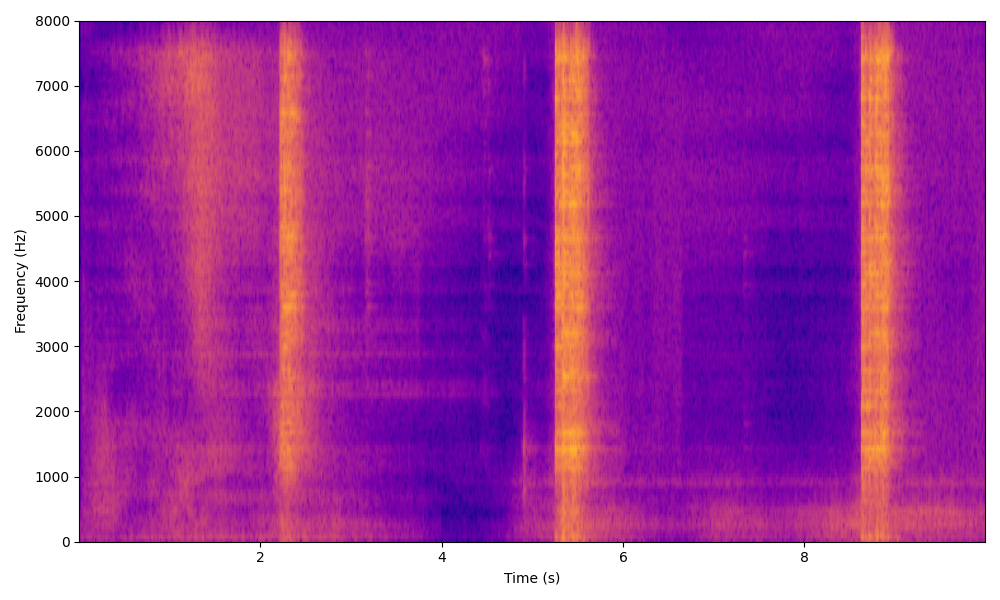
\includegraphics[width=\textwidth]{plots/onepeace_best_sdri/onepeace sep_spectrogram.png}
    \end{subfigure}
    \begin{subfigure}[b]{0.185\textwidth}
        \centering
        \includegraphics[width=\textwidth]{plots/onepeace_best_sdri/clap sep_spectrogram.png}
    \end{subfigure}
    \begin{subfigure}[b]{0.185\textwidth}
        \centering
        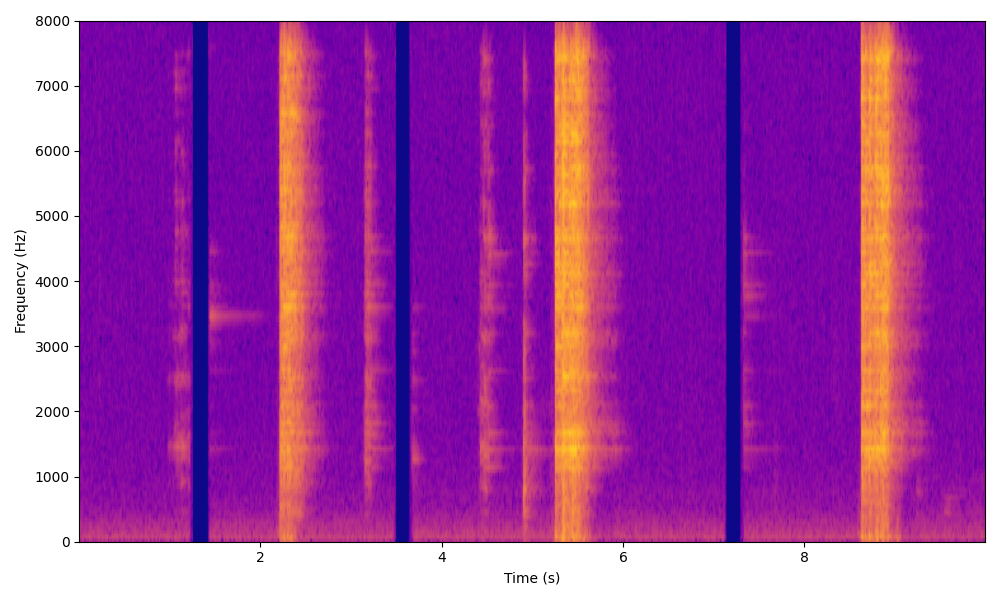
\includegraphics[width=\textwidth]{plots/onepeace_best_sdri/onepeace target_spectrogram.png}
    \end{subfigure}

    % Row 3 best onepeace delta_similarity improvement
     \begin{subfigure}[b]{0.185\textwidth}
        \centering
        \scriptsize\textbf{"Fireworks are shot into the air with swirling sounds and then they explode"}
        \vspace{5.0mm}
    \end{subfigure}
    \begin{subfigure}[b]{0.185\textwidth}
        \centering
        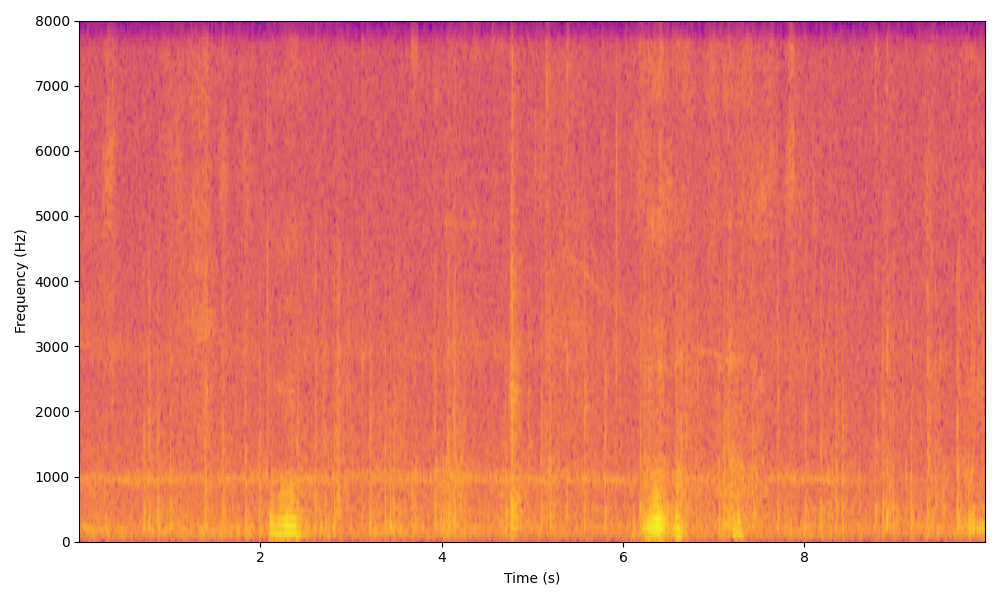
\includegraphics[width=\textwidth]{plots/onepeace_best_delta_similarity/onepeace mixture_spectrogram.png}
    \end{subfigure}
    \begin{subfigure}[b]{0.185\textwidth}
        \centering
        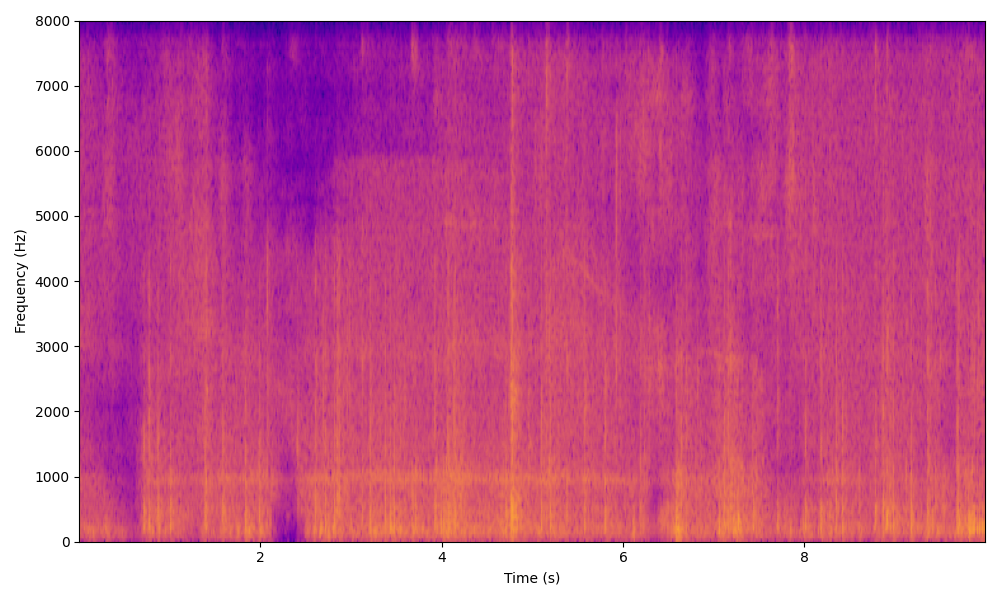
\includegraphics[width=\textwidth]{plots/onepeace_best_delta_similarity/onepeace sep_spectrogram.png}
    \end{subfigure}
    \begin{subfigure}[b]{0.185\textwidth}
        \centering
        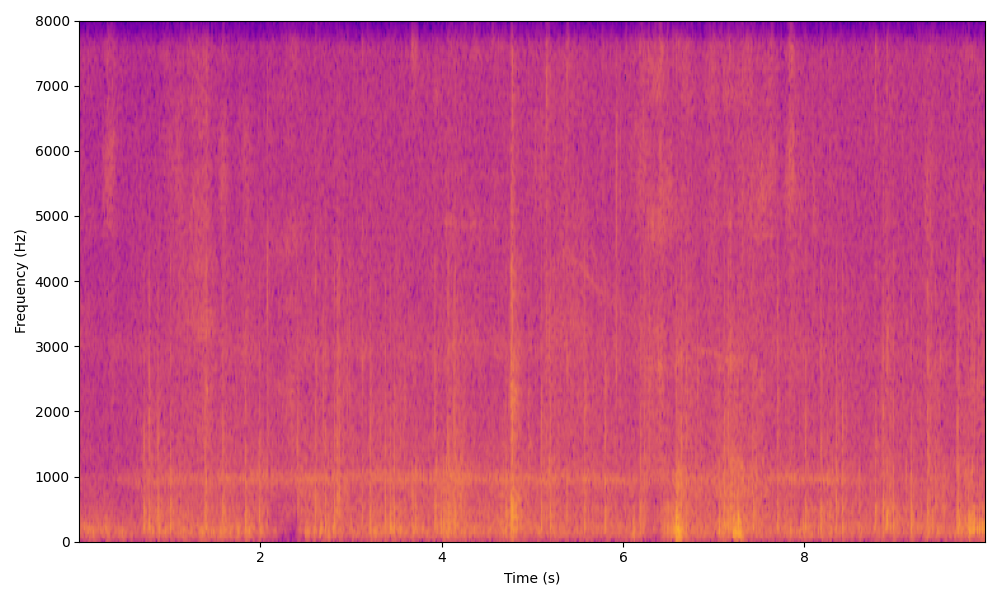
\includegraphics[width=\textwidth]{plots/onepeace_best_delta_similarity/clap sep_spectrogram.png}
    \end{subfigure}
    \begin{subfigure}[b]{0.185\textwidth}
        \centering
        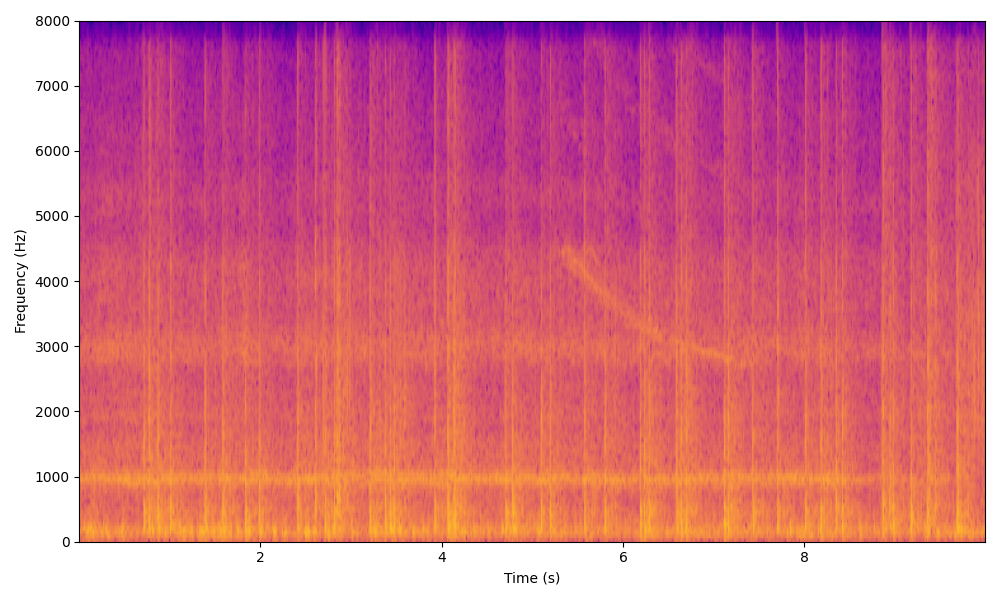
\includegraphics[width=\textwidth]{plots/onepeace_best_delta_similarity/onepeace target_spectrogram.png}
    \end{subfigure}

    % Row: high clap sdr, low onepeace sdr woosh_sound
    \begin{subfigure}[b]{0.185\textwidth}
        \centering
        \scriptsize\textbf{"A whooshing sound is moving rapidly"}
        \vspace{5.0mm}
        \caption*{Language Query}
    \end{subfigure}
    \begin{subfigure}[b]{0.185\textwidth}
        \centering
        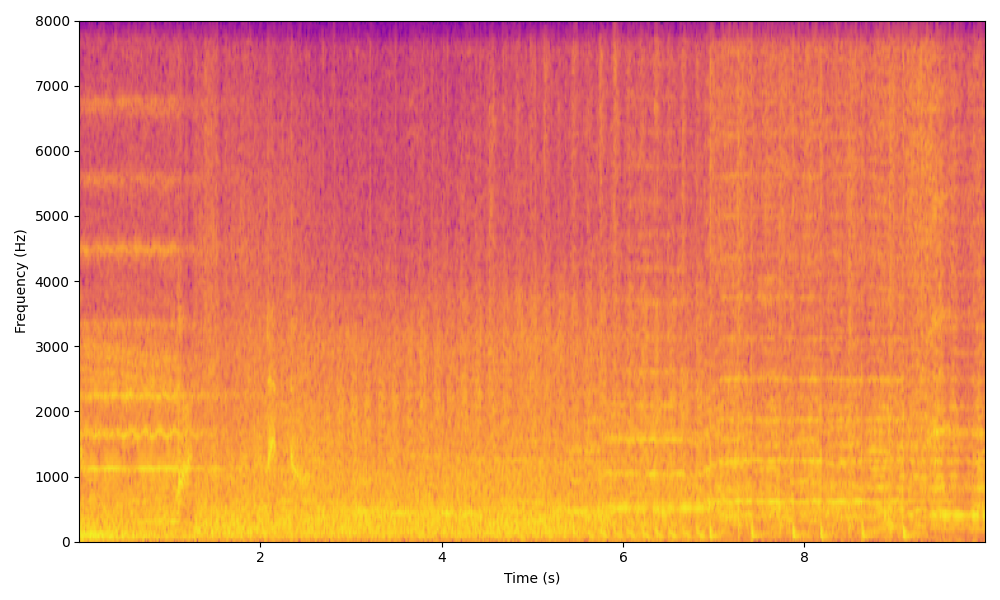
\includegraphics[width=\textwidth]{plots/whooshing_sound/clap mixture_spectrogram.png}
        \centering
        \caption*{Mixture}
    \end{subfigure}
    \begin{subfigure}[b]{0.185\textwidth}
        \centering
        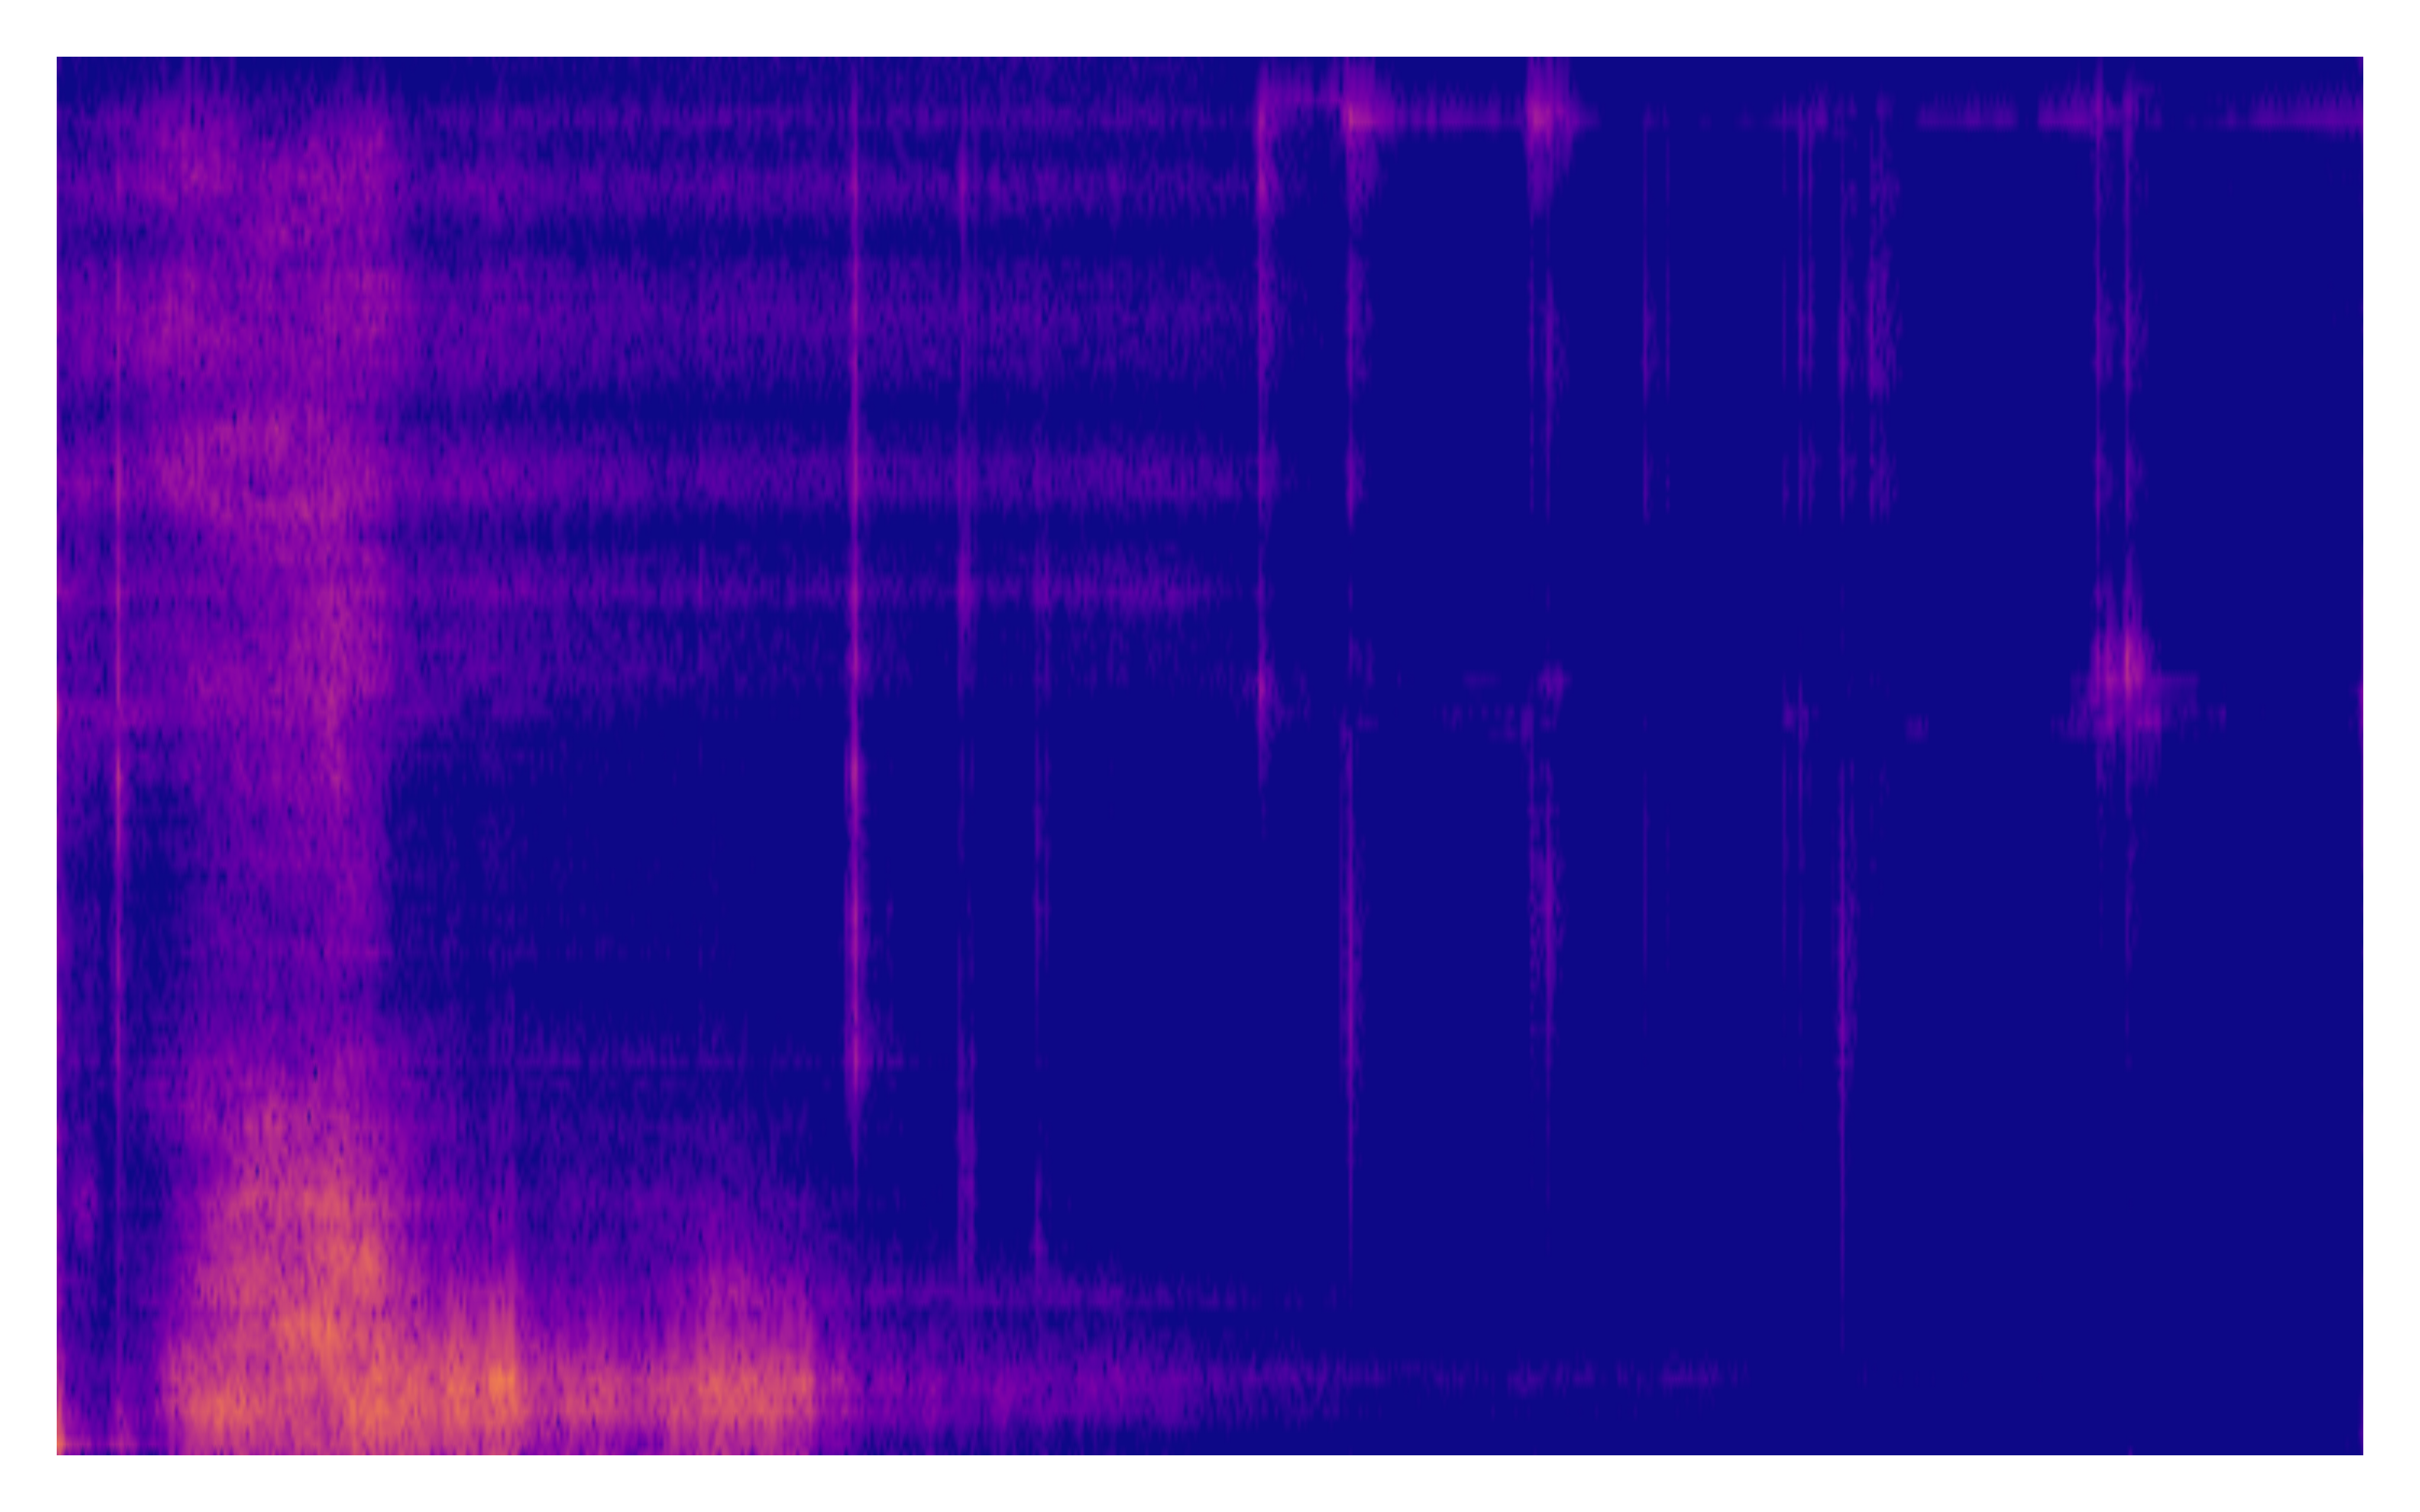
\includegraphics[width=\textwidth]{plots/whooshing_sound/onepeace sep_spectrogram.png}
        \caption*{ONE-PEACE}
    \end{subfigure}
    \begin{subfigure}[b]{0.185\textwidth}
        \centering
        \includegraphics[width=\textwidth]{plots/whooshing_sound/clap sep_spectrogram.png}
        \caption*{CLAP}
    \end{subfigure}
    \begin{subfigure}[b]{0.185\textwidth}
        \centering
        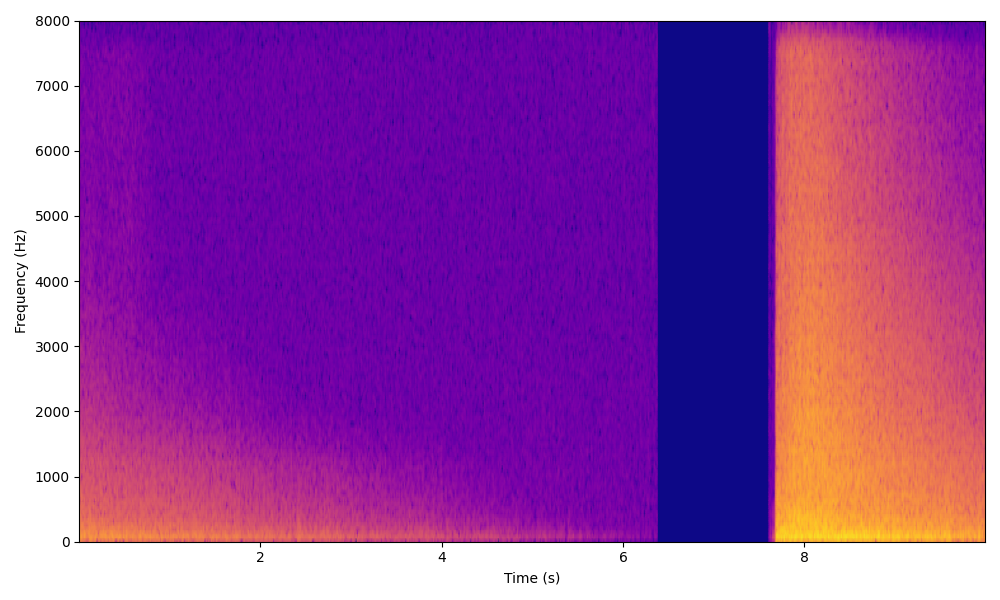
\includegraphics[width=\textwidth]{plots/whooshing_sound/clap target_spectrogram.png}
        \caption*{Target}
    \end{subfigure}
    
    % Continue rows similarly for other queries
    % Add caption below
    \caption{Visualized spectrograms for various language queries from the DCASE 2024 T9 Validation Set. The x-axis represents time, the y-axis represents the frequency of the signal, and the hue represents the power (decibels), where brighter colors have higher power.}
    
    \label{fig:separation_results}

\end{figure*}
